\documentclass{article}\usepackage{tikz}\begin{document}
\title{A TikZ gallery of basic examples}
\section{Connecting squares}
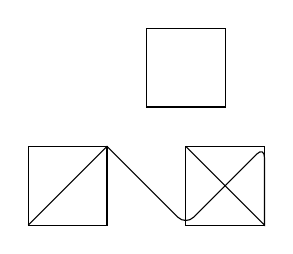
\begin{tikzpicture}
\draw (0,0) -- +(1,0) -- +(1,1) -- +(0,1) -- cycle;
\draw (2,0) -- +(1,0) -- +(1,1) -- +(0,1) -- cycle;
\draw (1.5,1.5) -- +(1,0) -- +(1,1) -- +(0,1) -- cycle;
\draw (0,0) -- (1,1) {[rounded corners] -- (2,0) -- (3,1)} -- (3,0) -- (2,1);
\end{tikzpicture}

\section{A Trapezoid with rounded corners}
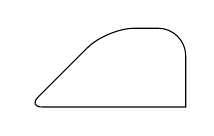
\begin{tikzpicture}
\draw (0,0) [rounded corners=10pt] -- (1,1) -- (2,1)
[sharp corners] -- (2,0)
[rounded corners=5pt] -- cycle;
\end{tikzpicture}

\section{A Unit Circle}
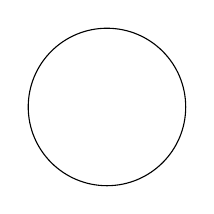
\begin{tikzpicture}
\draw[clip] (0,0) circle (1cm);
\end{tikzpicture}

\section{Plot of $\sin(x)$}
\begin{tikzpicture}
\draw plot (\x,{sin(\x r)});
\end{tikzpicture}

\section{Some plots}
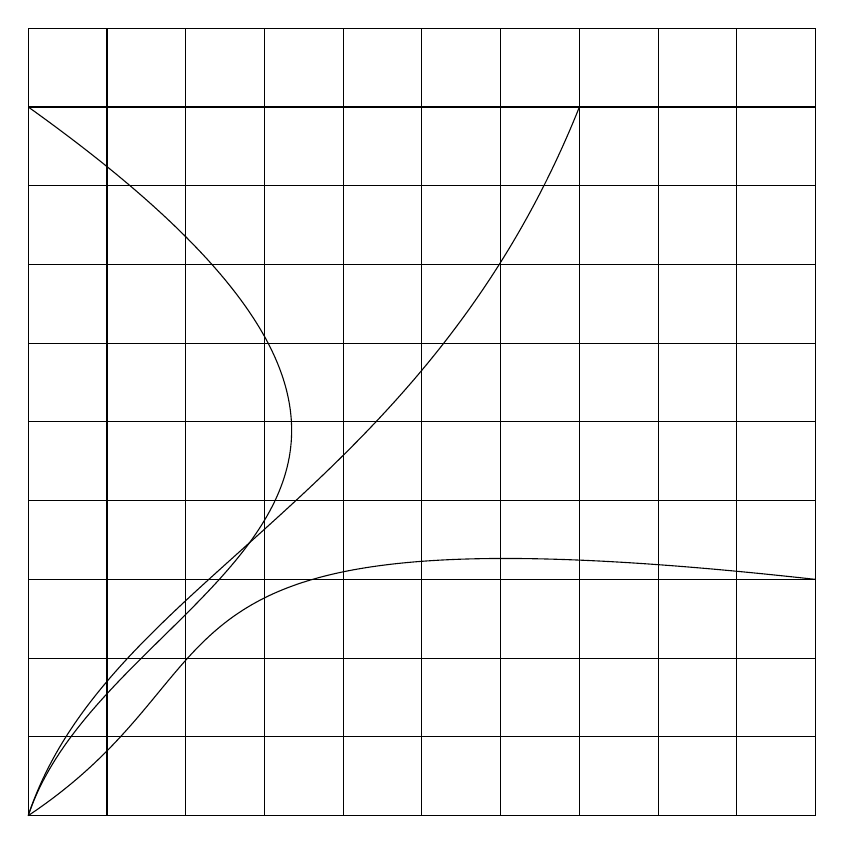
\begin{tikzpicture}
\draw (0,0) grid (10,10);
\pgfxycurve(0,0)(3,2)(1,4)(10,3)
\pgfstroke
\pgfxycurve(0,0)(1,3)(5,4)(7,9)
\pgfxycurve(0,0)(1,3)(7,4)(0,9)
\pgffill
\end{tikzpicture}\end{document}